\documentclass[table]{beamer}

\usetheme{Luebeck}
%\useinnertheme{circles}
\usepackage[utf8]{inputenc}
\usepackage{listings}

\title[CS225 Lab11: Reductions]{CS225 Lab11: Reductions with OpenMP}
\author{Chase Geigle}
\date{\today}
\institute{CS 225, UIUC}

\newcommand{\ttt}[1]{\begin{tt}#1\end{tt}}

\begin{document}
\frame{\titlepage}
\section{Overview}
\frame{\scriptsize\tableofcontents}

\section{Reductions}
\subsection{Motivation}

\begin{frame}[fragile]
    \frametitle{Motivating example: Finding a vector's sum}
    \begin{itemize}
        \item<1-> Consider the following code for finding the sum of the 
        integers in a vector.
        \begin{lstlisting}[language=C++]
int findSum( const vector<int> & list ) {
    int sum = 0;
    for( int i = 0; i < list.size(); i++ )
        sum += list[i];
    return sum;
}
        \end{lstlisting}
        \item<2-> Can this be parallelized?
        \item<3-> Not trivially. Why? What happens with the \ttt{sum} 
        variable?
    \end{itemize}
\end{frame}

 %\begin{frame}
 %    \frametitle{Down to the machine level}
 %    \begin{itemize}
 %        \item<1-> \ttt{sum += list[i]}
 %        \item<2-> Translates into assembly language (and then machine 
 %        language) as \textbf{multiple statements}!
 %        \item<3-> Pseudo-assembly translation:\newline
 %        \rowcolors{0}{blue!20}{blue!40}
 %        \begin{tabular}{ll}
 %        load r1, sum \\
 %        load r2, list[i]    \onslide<5->{& load r1, sum}\\
 %        add r3, r1, r2      \onslide<5->{& load r2, list[i]}\\
 %        store r3, sum       \onslide<5->{& add r3, r1, r2}\\
 %        \quad               \onslide<5->{& store r3, sum}
 %        \end{tabular}
 %        \item<4-> What happens if we interleave these assembly statements?  
 %        (i.e., what happens if we run with multiple threads?)
 %        \item<6-> We no longer get the correct result---we caused a 
 %        \textbf{race condition}.
 %    \end{itemize}
 %\end{frame}
 
 \begin{frame}
    \frametitle{Down to the machine level}
    \begin{itemize}
        \item<1-> \ttt{sum += list[i]} translates to \textbf{multiple
        instructions} in machine code.
        \item<2-> Each CPU core (which runs a thread) can only perform
        arithmetic on things that are currently loaded in.
        \item<3-> Need to load in \ttt{sum} and \ttt{list[i]} before they
        can be added.
        \item<4-> Then the result must be stored back into memory.
        \item<5-> But why is this a problem? What happens if we interleave
        these multiple machine instructions?
    \end{itemize}
 \end{frame}

\begin{frame}
    \only<1>{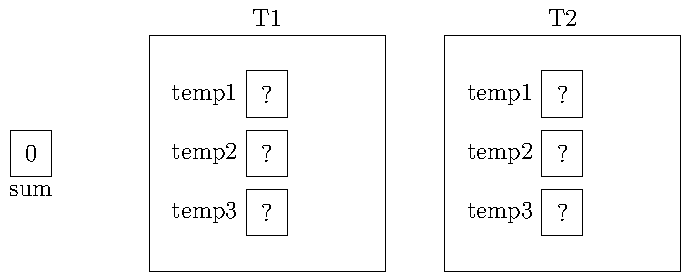
\includegraphics{thread_diagram1.pdf}}
    \only<2>{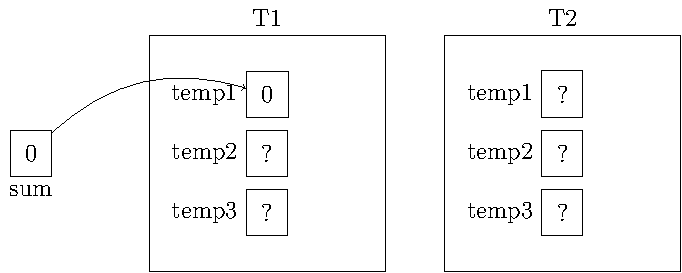
\includegraphics{thread_diagram2.pdf}}
    \only<3>{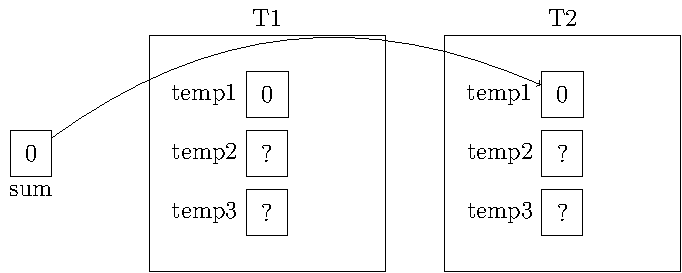
\includegraphics{thread_diagram3.pdf}}
    \only<4>{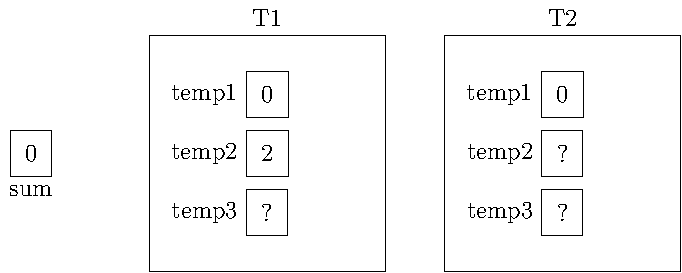
\includegraphics{thread_diagram4.pdf}}
    \only<5>{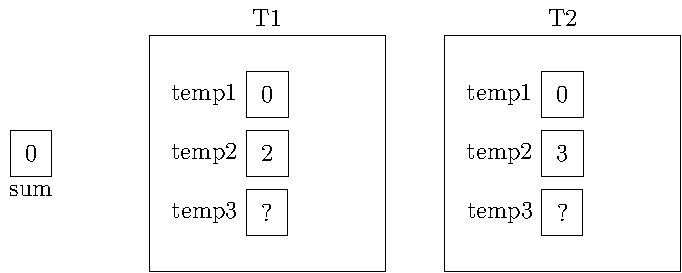
\includegraphics{thread_diagram5.pdf}}
    \only<6>{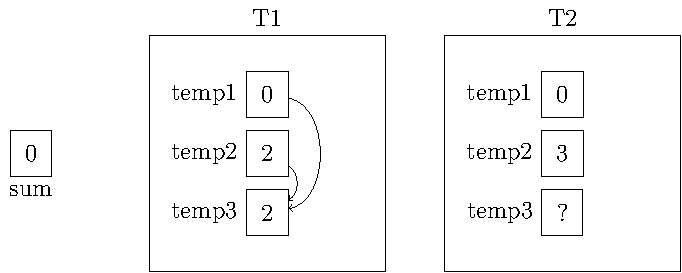
\includegraphics{thread_diagram6.pdf}}
    \only<7>{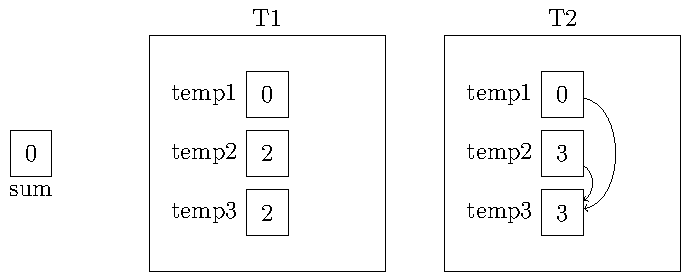
\includegraphics{thread_diagram7.pdf}}
    \only<8>{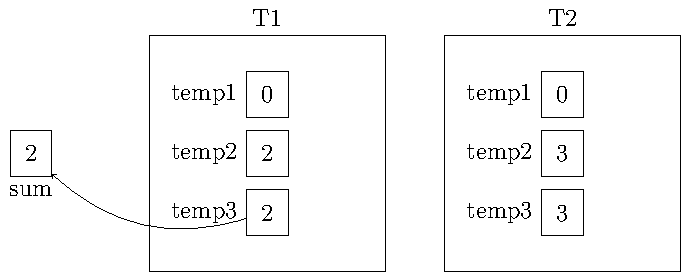
\includegraphics{thread_diagram8.pdf}}
    \only<9>{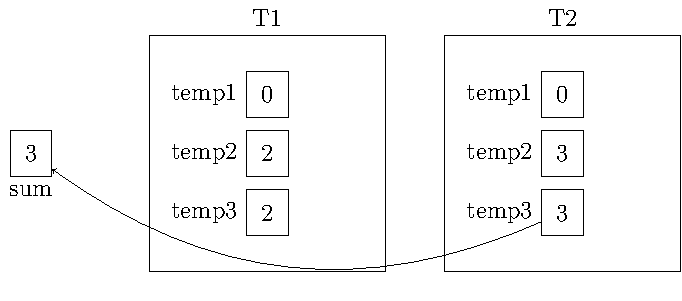
\includegraphics{thread_diagram9.pdf}}
\end{frame}


\begin{frame}
    \frametitle{Parallelizing the vector sum problem}
    \begin{itemize}
        \item<1-> Suppose you have $t$ threads, and you know the answer to 
        your $t$ parallel subproblems (each thread's result for its section 
        of the vector) is the set $T$.
        \item<2-> How can the final answer be computed?
        \only<1-2>{\vspace{2.5cm}}
        \only<3->{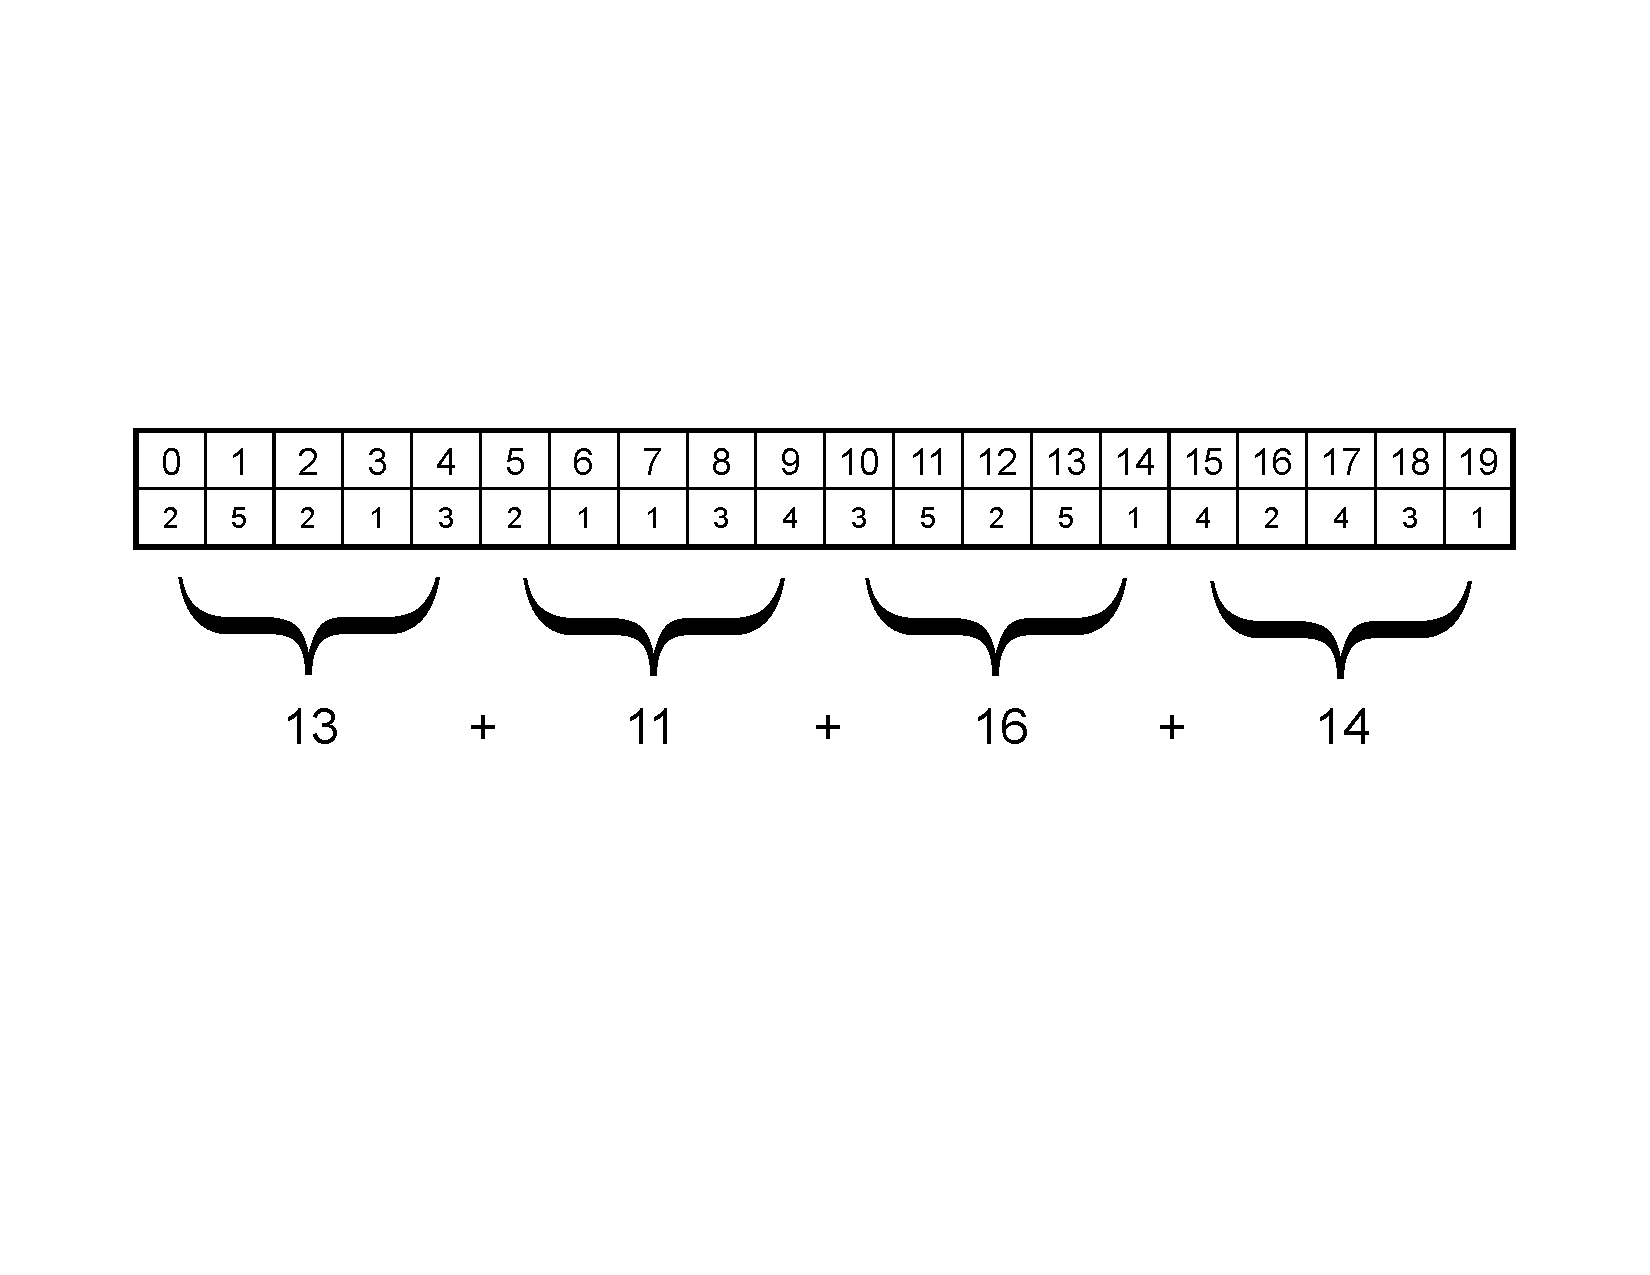
\includegraphics[scale=.4]{lab11-1dsumexample.pdf}}
        \item<4-> $\sum_{\forall a\in T}(a)$ (that is, sum up the values in
        $T$)
        \item<5-> This step is an example of a \emph{reduction}.
    \end{itemize}
\end{frame}

\subsection{Definition}
\begin{frame}
    \frametitle{Reductions}
    \begin{definition}
        \begin{itemize}
            \item<1-> A \emph{reduction} is an operation applied to an
            array to produce a result of a lesser rank.
            \item<2-> In our example, we have an array of results, $T$ from
            each thread's subproblem.
            \item<3-> If $x$ is the answer computed in a parallel subproblem, 
            we run a ``reduction on $x$'' to get our final answer.
        \end{itemize}
    \end{definition}
    % removed because it's TOO DEEP FOR YOU
    % \begin{itemize}
    %     \item<3-> Food for thought: can you always do reductions if $x\in 
    %     \mathbb{R}$?
    %     \item<4-> What mathematical property must the reduction operation 
    %     have?
    % \end{itemize}
\end{frame}

\begin{frame}
    \frametitle{Reductions in OpenMP}
    \begin{itemize}
        \item<1-> How do we write reductions in OpenMP?
        \item<2-> In general, we have two options:
        \begin{enumerate}
            \item<3-> Use an OpenMP feature called the ``reduction 
            clause''.
            \begin{itemize}
                \item<4-> This is a useful shorthand, but it isn't always 
                an option for more complicated reduction statements.
            \end{itemize}
            \item<5-> Manually fix the race condition on the reduction 
            variable.
            \begin{itemize}
                \item<6-> This is always an option, regardless of the 
                complexity of the reduction statement.
            \end{itemize}
        \end{enumerate}
    \end{itemize}
\end{frame}

\subsection{Critical Regions}
\begin{frame}
    \frametitle{Critical Regions and Atomicity}
    \begin{definition}
        An \textbf{atomic} operation is one that happens entirely in one 
        step.
    \end{definition}
    \onslide<2->{
    \begin{definition}
        A \textbf{critical region} is a section of code whose operation 
        must be \textbf{atomic} for correctness. Critical regions that are 
        not safeguarded are often the root causes of race conditions.
    \end{definition}
    }
    \begin{itemize}
        \item<3-> We guarantee critical regions are \textbf{atomic} by only 
        allowing one thread to execute in the critical region at a time.
        \item<4-> How can we use the idea of a ``critical region'' to help 
        manually fix the race condition on the \ttt{sum} variable?
    \end{itemize}
\end{frame}

\subsection{Applications}
\begin{frame}[fragile]
    \frametitle{Example: Manual Reduction With a Critical Region}
\begin{lstlisting}[language=C++]
int findSum(const vector<int> & list) {
  int sum = 0;
  #pragma omp parallel
  {
    int local_sum = 0;
    #pragma omp for
    for( int i = 0; i < list.size(); i++ )
      local_sum += list[i];
    #pragma omp critical
    sum += local_sum;
  }
  return sum;
}
\end{lstlisting}
\end{frame}

\begin{frame}[fragile]
    \frametitle{Un-fuzzying the example}
    \begin{columns}[c]
        \column{1.8in}
        \scriptsize What are the pragmas here doing?
\begin{lstlisting}[language=C++,basicstyle=\tiny]
int findSum(const vector<int> & list) {
  int sum = 0;
  #pragma omp parallel
  {
    int local_sum = 0;
    #pragma omp for
    for( int i = 0; i < list.size(); i++ )
      local_sum += list[i];
    #pragma omp critical
    sum += local_sum;
  }
  return sum;
}
\end{lstlisting}
        \column{2.8in}
        \begin{itemize}
        \item<2-> \scriptsize\ttt{omp parallel}
        \begin{itemize}
            \item<3-> \scriptsize Creates a team of threads to operate on 
            the given block (a block is between \ttt{\{\}}).
        \end{itemize}
        \item<4-> \scriptsize\ttt{omp for}
        \begin{itemize}
            \item<5-> \scriptsize Parallelizes a for loop, using the team 
            of threads that exist at this point.
            \item<6-> \scriptsize Note that we omit the \ttt{parallel} 
            directive here because we already have spawned a team of 
            threads.
        \end{itemize}
        \item<7-> \scriptsize\ttt{omp critical}
        \begin{itemize}
            \item<8-> \scriptsize Designates the given block of code as a 
            ``critical region''.
            \item<9-> \scriptsize Only one thread in the team is allowed to 
            be executing in the critical region at a time.
            \item<10-> \scriptsize This fixes our race condition!
        \end{itemize}
    \end{itemize}
    \end{columns}
\end{frame}

\begin{frame}[fragile]
    \frametitle{Execution Diagram}
    What does this look like when running?
    \begin{columns}[c]
        \column{2.6in}
\begin{lstlisting}[language=C++,basicstyle=\tiny]
int findSum(const vector<int> & list) {
  int sum = 0;
  #pragma omp parallel
  {
    int local_sum = 0;
    #pragma omp for
    for( int i = 0; i < list.size(); i++ )
      local_sum += list[i];
    #pragma omp critical
    sum += local_sum;
  }
  return sum;
}
\end{lstlisting}

        \column{1.8in}
        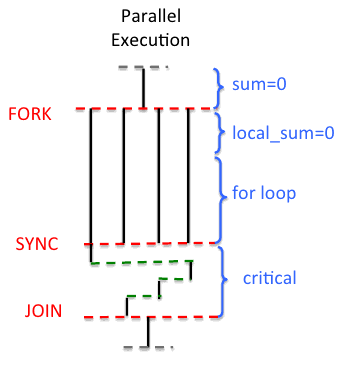
\includegraphics[scale=.4]{execution_diagram.png}
    \end{columns}
\end{frame}

\begin{frame}[fragile]
    \frametitle{The Reduction Clause}
    In this example, we can apply the ``reduction clause'' to simplify our 
    code.
    \begin{itemize}
        \item<2-> The ``reduction clause'' comes after a for construct and 
        takes the form \ttt{reduction(operator: variables)}.
        \item<3-> The \ttt{operator} can only be of the following: $+$, 
        $*$, $-$, $/$, $\&$, $\verb|^|$, $|$, $\&\&$, $||$.
        \item<4-> It \emph{cannot be overloaded}.
        \item<5-> The elements provided as \ttt{variables} must be scalar (primitive) types.
    \end{itemize}
\end{frame}

\begin{frame}[fragile]
    \frametitle{Example: Using the Reduction Clause}
\begin{lstlisting}[language=C++]
int findSum( const vector<int> & list ) {
    int sum = 0;
    #pragma omp parallel for reduction(+: sum)
    for( int i = 0; i < list.size(); i++ )
        sum += list[i];
    return sum;
}
\end{lstlisting}
    \pause
    This is shorthand for resolving the race condition manually.
\end{frame}

\begin{frame}[fragile]
    \frametitle{Another Example: Largest Integer Problem}
    \begin{itemize}
        \item<1-> Consider the code below for finding the maximum integer 
        in an array.
\begin{lstlisting}[language=C++,basicstyle=\scriptsize]
int findMax( const vector<int> & list ) {
    int max = INT_MIN;
    for( int i = 0; i < list.size(); i++ )
        if( max < list[i] )
            max = list[i];
    return max;
}
\end{lstlisting}
        \item<2-> Can this be parallelized?
        \item<3-> What reduction method will you use?
        \item<4-> Why aren't we able to use a reduction clause here?
        \item<5-> Full disclosure: This will eventually be possible with a 
        reduction clause in OpenMP 3.1 (supported in GCC 4.7).
    \end{itemize}
\end{frame}

% the next several frames are for showing bits of code incrementally, since 
% the listings environment doesn't appear to support \only<X->

\begin{frame}[fragile]
    \frametitle{Parallelizing the Maximum Integer Problem}
    Filling in the code:
\begin{lstlisting}[language=C++,basicstyle=\scriptsize]
int findMax( const vector<int> & list ) {
    int max = INT_MIN;

    {
        int local_max = max;

        for( int i = 0; i < list.size(); i++ )
            if( local_max < list[i] )
                local_max = list[i];

        {


        }
    }
    return max;
}
\end{lstlisting}
\end{frame}

\begin{frame}[fragile]
    \frametitle{Parallelizing the Maximum Integer Problem}
    Filling in the code:
\begin{lstlisting}[language=C++,basicstyle=\scriptsize]
int findMax( const vector<int> & list ) {
    int max = INT_MIN;
    #pragma omp parallel
    {
        int local_max = max;

        for( int i = 0; i < list.size(); i++ )
            if( local_max < list[i] )
                local_max = list[i];

        {


        }
    }
    return max;
}
\end{lstlisting}
\end{frame}

\begin{frame}[fragile]
    \frametitle{Parallelizing the Maximum Integer Problem}
    Filling in the code:
\begin{lstlisting}[language=C++,basicstyle=\scriptsize]
int findMax( const vector<int> & list ) {
    int max = INT_MIN;
    #pragma omp parallel
    {
        int local_max = max;
        #pragma omp for
        for( int i = 0; i < list.size(); i++ )
            if( local_max < list[i] )
                local_max = list[i];

        {


        }
    }
    return max;
}
\end{lstlisting}
\end{frame}

\begin{frame}[fragile]
    \frametitle{Parallelizing the Maximum Integer Problem}
    Filling in the code:
\begin{lstlisting}[language=C++,basicstyle=\scriptsize]
int findMax( const vector<int> & list ) {
    int max = INT_MIN;
    #pragma omp parallel
    {
        int local_max = max;
        #pragma omp for
        for( int i = 0; i < list.size(); i++ )
            if( local_max < list[i] )
                local_max = list[i];
        #pragma omp critical
        {


        }
    }
    return max;
}
\end{lstlisting}
\end{frame}

\begin{frame}[fragile]
    \frametitle{Parallelizing the Maximum Integer Problem}
    Filling in the code:
\begin{lstlisting}[language=C++,basicstyle=\scriptsize]
int findMax( const vector<int> & list ) {
    int max = INT_MIN;
    #pragma omp parallel
    {
        int local_max = max;
        #pragma omp for
        for( int i = 0; i < list.size(); i++ )
            if( local_max < list[i] )
                local_max = list[i];
        #pragma omp critical
        {
            if( max < local_max )
                max = local_max;
        }
    }
    return max;
}
\end{lstlisting}
\end{frame}

\begin{frame}
    \frametitle{Aside: When to use the Reduction Clause}
    \begin{itemize}
        \item<1-> In general, the reduction clause can only be used if our 
        reduction is a simplistic one.
        \item<2-> For more complicated reductions (such as ones involving 
        2D arrays or more interesting data structures), we will have to 
        write a manual reduction.
    \end{itemize}
\end{frame}

\section{Map Reduce}
\begin{frame}
    \frametitle{Map Reduce}
    \begin{itemize}
        \item<1-> What we have seen so far is a generalization of the Map 
        Reduce pattern.
        \item<2-> \textbf{Map Reduce} was introduced by Google in 2004 as a 
        way of processing large amounts of data in parallel.
        \item<3-> Uses a cluster of machines to do the processing.
        \item<4-> Broken into two steps:
        \begin{itemize}
            \item<5-> Map: Partition the input into small pieces, and run a 
            function (\ttt{map()}) on each piece. The result is a list of 
            (key, value) pairs.
            \item<6-> Reduce: Combines many lists produced from each Map 
            step into a smaller set of (key, value) pairs.
        \end{itemize}
        \item<7-> In our examples, our \ttt{parallel for} directive is our 
        mapping function, and our reduction setup is the reduce step.
    \end{itemize}
\end{frame}

\section{Summary}
\begin{frame}
    \frametitle{Summary}
    So what have we seen?
    \begin{itemize}
        \item<1-> \textbf{Race conditions} are a big concern when writing 
        parallel code.
        \item<2-> \textbf{Reductions} can help us assemble a main result 
        from a list of results of parallel subproblems.
        \item<3-> There is a subset of Race conditions that can be resolved 
        by using \textbf{reductions}.
        \item<4-> The general paradigm in use here is the same as that used 
        in \textbf{Mapreduce}!
    \end{itemize}
\end{frame}

\end{document}
